\documentclass[journal,article,submit,pdftex,moreauthors]{Definitions/mdpi} 

\Title{EcoActivity: Aplikasi Rekomendasi Aktivitas Berbasis Cuaca}

% MDPI internal command: Title for citation in the left column
\TitleCitation{EcoActivity: Aplikasi Rekomendasi Aktivitas Berbasis Cuaca}

% Authors, for the paper (add full first names)
\Author{Kevin Al Gazali $^{1}$, Shaff Shalihin $^{1}$, Vicky Jesflinto $^{1}$, Ahmad Fauzhan Ramadhan $^{1}$, Zefanya Farrel Palinggi $^{1}$, Muh.Shofwan Siswandi $^{1/2}
}
%\longauthorlist{yes}

% MDPI internal command: Authors, for metadata in PDF
\AuthorNames{Kevin Al Gazali, Shaff Shalihin, Vicky Jesflinto, Ahmad Fauzhan Ramadhan, Zefanya Farrel Palinggi, Muh. Shofwan Siswandi}

% MDPI internal command: Authors, for citation in the left column
\AuthorCitation{Gazali, K. A.; Shalihin, S.; Jesflinto, V.; Ramadhan, A. F.; Palinggi, Z. F.; Siswandi, M. S.}
% If this is a Chicago style journal: Lastname, Firstname, Firstname Lastname, and Firstname Lastname.

% Affiliations / Addresses (Add [1] after \address if there is only one affiliation.)
\address{%
$^{1}$ \quad Universitas Hasanuddin; gazalika22h@student.unhas.ac.id, shalihins22h@student.unhas.ac.id, jesflintov22h@student.unhas.ac.id, bafr22h@student.unhas.ac.id, palinggizf22h@student.unhas.ac.id, siswandims20h@student.unhas.ac.id\\
}
% Contact information of the corresponding author
\corres{Correspondence: gazalika22h@student.unhas.ac.id;Tel.: +62 822-6064-0071}

% Current address and/or shared authorship
\firstnote{Current address: Jalan Perintis Kemerdekaan Km. 10 Tamalanrea, Kota:Makassar}  % Current address should not be the same as any items in the Affiliation section.
% The commands \thirdnote{} till \eighthnote{} are available for further notes
\thirdnote{These authors contributed equally to this work.}
%\simplesumm{} % Simple summary

%\conference{} % An extended version of a conference paper

% Abstract (Do not insert blank lines, i.e. \\) 
\abstract{Cuaca memiliki pengaruh yang signifikan terhadap aktivitas harian manusia. Dengan perkembangan teknologi, aplikasi berbasis cuaca dapat membantu pengguna memilih aktivitas yang sesuai dengan kondisi cuaca terkini. Penelitian ini bertujuan untuk mengembangkan aplikasi EcoActivity yang memberikan daftar kegiatan berdasarkan prediksi apakah aktivitas tersebut lebih cocok dilakukan di dalam ruangan atau di luar ruangan. Aplikasi ini memanfaatkan data cuaca real-time yang diperoleh melalui API cuaca dan diproses menggunakan algoritma pembelajaran mesin untuk menentukan prediksi indoor atau outdoor berdasarkan parameter seperti suhu, kelembapan, kecepatan angin, curah hujan, indeks UV, dan visibilitas. Sistem ini memberikan list kegiatan yang sesuai dengan prediksi cuaca, seperti kegiatan dalam ruangan saat cuaca buruk atau kegiatan luar ruangan saat cuaca cerah. Hasil pengujian menunjukkan bahwa aplikasi mampu memberikan daftar kegiatan yang relevan berdasarkan kondisi cuaca saat itu. Pengujian antarmuka pengguna mengungkapkan bahwa aplikasi ini mudah digunakan dan responsif. EcoActivity menunjukkan potensi besar dalam membantu pengguna memilih aktivitas yang sesuai dengan kondisi cuaca. Aplikasi ini dapat dikembangkan lebih lanjut dengan menambahkan fitur tambahan, seperti integrasi data cuaca jangka panjang atau analisis prediksi berbasis lokasi..
}

% Keywords
\keyword{Cuaca; Aplikasi; Pembelajaran Mesin; Sistem Cerdas; Teknologi Cuaca; Sistem Informasi} 
\usepackage{graphicx} % Untuk menyisipkan gambar
\usepackage{subcaption} % Untuk sub-gambar
\usepackage{float}
\renewcommand{\figurename}{Gambar}
\begin{document}
\section{Project Charter}

\subsection{Project Title}
Proyek EcoActivity bertujuan untuk mengembangkan sebuah aplikasi pintar yang memberikan daftar kegiatan berdasarkan prediksi apakah aktivitas tersebut lebih cocok dilakukan di dalam ruangan atau di luar ruangan, sesuai dengan kondisi cuaca terkini. Aplikasi ini memungkinkan pengguna untuk merencanakan kegiatan sehari-hari dengan lebih baik dengan memanfaatkan data cuaca real-time dan algoritma pembelajaran mesin yang adaptif. Tujuan utama proyek ini adalah: \begin{itemize} 
\item Menyediakan daftar kegiatan harian yang sesuai dengan prediksi indoor atau outdoor berdasarkan kondisi cuaca. 
\item Mengintegrasikan data cuaca real-time dari API eksternal untuk memberikan informasi yang akurat. 
\item Mengembangkan antarmuka pengguna yang responsif dan mudah digunakan. 
\end{itemize}

\subsection{Scope of the Project}

Ruang lingkup proyek EcoActivity mencakup: \begin{itemize} 
\item Pengembangan aplikasi berbasis Android Studio sebagai antarmuka pengguna. 
\item Integrasi dengan API cuaca eksternal (Tomorrow API) untuk data cuaca terkini.
\item Penyediaan fitur daftar kegiatan yang disesuaikan dengan prediksi indoor atau outdoor berdasarkan kondisi cuaca terkini. 
\item Pengujian antarmuka pengguna untuk memastikan aplikasi mudah digunakan dan responsif.

\end{itemize}

\subsection{Project Team}

Tim proyek EcoActivity terdiri dari enam anggota dengan peran berikut:
\begin{itemize}
    \item Kevin Al Gazali : UI/UX Designer.
    \item Shaff Shalihin : Backend Developer.
    \item Zefanya Farrel : Backend Developer.
    \item Muh.Shofwan Siswandi : Backend Developer.
    \item Vicky Jesflinto : Frontend Developer.
    \item Ahmad Fauzan Ramadhan : Frontend Developer.
\end{itemize}
\subsection{Project Milestones and Timeline}

Berikut adalah tonggak penting dan garis waktu yang direncanakan untuk proyek EcoActivity:
\begin{itemize}
    \item Perencanaan - Minggu 1-4
    \item Pengumpulan Data - Minggu 5-6
    \item Pengembangan - Minggu 7-10
    \item Pengujian - Minggu 11-14
    \item Deployment - Minggu 15
    \item Pengujian dan Validasi Sistem - Minggu 13-14
    \item Penyusunan Laporan - Minggu 16
\end{itemize}
\subsection{Assumptions and Constraints}

Proyek EcoActivity bergantung pada asumsi dan batasan berikut: \begin{itemize} 
\item Ketersediaan akses API cuaca eksternal untuk data cuaca real-time yang akurat. 
\item Akurasi daftar kegiatan terbatas oleh kualitas data cuaca terkini yang diterima dari API eksternal. \item Aplikasi harus user-friendly dan responsif untuk pengguna tanpa latar belakang teknis. 
\end{itemize}

\subsection{Risks and Mitigations}

Beberapa risiko yang diidentifikasi beserta langkah mitigasinya adalah sebagai berikut: 
\begin{itemize} 
\item Keterbatasan Data Cuaca: Jika data cuaca sulit diakses, API alternatif akan dicari untuk memastikan kelancaran aliran data real-time. 
\item Ketidakakuratan Daftar Kegiatan: Sistem akan diuji secara berkelanjutan dan disesuaikan berdasarkan umpan balik pengguna untuk meningkatkan relevansi prediksi indoor atau outdoor. 
\item Masalah Integrasi API: Prosedur debugging dan pengujian integrasi API akan dilakukan secara menyeluruh, dan dokumentasi API akan dikaji untuk memastikan kelancaran penggunaan. 
\end{itemize}

%%%%%%%%%%%%%%%%%%%%%%%%%%%%%%%%%%%%%%%%%%
\section{Materials and Methods}

Bagian ini menjelaskan metode yang digunakan dalam pengembangan dan evaluasi aplikasi EcoActivity. Proyek ini bertujuan untuk memberikan daftar aktivitas yang disesuaikan dengan kondisi cuaca terkini. Aplikasi ini mengandalkan data cuaca real-time yang diperoleh melalui API cuaca dan diproses menggunakan algoritma pembelajaran mesin untuk memprediksi apakah aktivitas yang sesuai adalah indoor atau outdoor.


\subsection{Data Collection and Explanation}
Data yang digunakan dalam aplikasi EcoActivity diperoleh dari tiga sumber utama yaitu :
\begin{itemize}
    \item Tomorrow API : API ini menyediakan data cuaca real-time yang mencakup parameter seperti suhu, kelembapan, kecepatan angin, dan kondisi cuaca (misalnya cerah, hujan, berawan), yang digunakan untuk memperbarui kondisi cuaca dalam aplikasi.
    \item Dataset weather type classification dari Kaggle: Dataset ini berguna untuk melatih algoritma klasifikasi, praktik preprocessing data, teknik deteksi outlier, dan analisis data cuaca.
    \item Dataset Aktivitas dan Parameter Cuaca: Dataset ini berisi data parameter cuaca seperti suhu, kelembapan, kecepatan angin, curah hujan, indeks UV, visibilitas, dan lainnya, yang dipasangkan dengan kategori aktivitas (Activity Category), yaitu Indoor atau Outdoor. Data ini digunakan untuk melatih dan mengevaluasi model prediksi dalam aplikasi EcoActivity.
\end{itemize}

\subsection{Algorithm or Model}

Aplikasi \textbf{EcoActivity} memanfaatkan integrasi dengan API cuaca untuk memberikan daftar aktivitas berdasarkan kondisi cuaca terkini. 

\subsubsection*{Prediksi Aktivitas Berdasarkan Data Cuaca Real-Time}
Aplikasi terhubung dengan \textit{Tomorrow API} untuk mendapatkan data cuaca real-time, termasuk parameter seperti suhu (\textit{temperature}), kelembapan (\textit{humidity}), kecepatan angin (\textit{wind speed}), curah hujan (\textit{precipitation}), indeks UV (\textit{UV index}), dan visibilitas (\textit{visibility}). Berdasarkan data cuaca yang diterima, sistem memprediksi apakah kondisi lebih cocok untuk aktivitas dalam ruangan (\textit{indoor}) atau luar ruangan (\textit{outdoor}).

Sebagai contoh:
\begin{itemize}
    \item Jika data menunjukkan cuaca cerah dengan kelembapan rendah dan curah hujan rendah, aplikasi akan memberikan daftar aktivitas luar ruangan.
    \item Jika data menunjukkan curah hujan tinggi dan visibilitas rendah, aplikasi akan memberikan daftar aktivitas dalam ruangan.
\end{itemize}

\subsubsection*{Penggunaan Random Forest sebagai Model Prediksi}
Untuk meningkatkan akurasi prediksi, aplikasi menggunakan algoritma \textit{Random Forest}, yaitu model pembelajaran mesin berbasis \textit{ensemble} yang mengandalkan kombinasi banyak pohon keputusan (\textit{decision trees}) untuk membuat prediksi yang lebih akurat dan stabil.

\paragraph{Langkah-Langkah Implementasi:}
\begin{enumerate}
    \item \textbf{Persiapan Data}: 
    Dataset disiapkan dengan fitur-fitur cuaca seperti suhu (\textit{temperature}), kelembapan (\textit{humidity}), kecepatan angin (\textit{wind speed}), curah hujan (\textit{precipitation}), indeks UV (\textit{UV index}), dan visibilitas (\textit{visibility}). Label target ditentukan sebagai \textbf{Indoor (1)} untuk aktivitas dalam ruangan dan \textbf{Outdoor (0)} untuk aktivitas luar ruangan.
    
    \item \textbf{Pelatihan Model}:
    Data dibagi menjadi dua bagian, yaitu data pelatihan (\textit{training data}) dan data pengujian (\textit{testing data}). Model \textit{Random Forest} dilatih dengan data pelatihan menggunakan beberapa pohon keputusan yang dibangun berdasarkan subset acak dari data dan fitur.
    
    \item \textbf{Prediksi dan Evaluasi}:
    Model digunakan untuk memprediksi kelas aktivitas (Indoor atau Outdoor) berdasarkan data cuaca real-time. Evaluasi dilakukan menggunakan metrik seperti \textit{precision}, \textit{recall}, \textit{F1-score}, dan \textit{accuracy}.
\end{enumerate}

\paragraph{Keunggulan Random Forest untuk EcoActivity:}
\begin{itemize}
    \item \textbf{Kemampuan Generalisasi}: 
    Random Forest memanfaatkan banyak pohon untuk mengurangi risiko \textit{overfitting}, sehingga cocok untuk data cuaca yang bersifat dinamis.
    
    \item \textbf{Efisiensi dengan Data Multivariat}: 
    Algoritma ini dapat menangani berbagai parameter cuaca sekaligus dan menentukan fitur mana yang paling relevan dalam mempengaruhi prediksi.
    
    \item \textbf{Stabilitas Model}: 
    Dengan pendekatan \textit{ensemble}, model memberikan hasil yang lebih konsisten bahkan jika data pelatihan memiliki variasi.
\end{itemize}

\paragraph{Implementasi Prediksi di Aplikasi:}
Data cuaca real-time yang diperoleh dari \textit{Tomorrow API} digunakan sebagai input untuk model \textit{Random Forest}. Model ini menghasilkan prediksi apakah aktivitas lebih cocok dilakukan di dalam atau luar ruangan. Prediksi ini kemudian digunakan untuk memberikan rekomendasi aktivitas yang sesuai kepada pengguna.

Dengan pendekatan ini, aplikasi \textbf{EcoActivity} dapat memberikan solusi berbasis data yang membantu pengguna memilih aktivitas sesuai dengan kondisi cuaca terkini secara akurat dan efisien.

\subsection{Testing (Procedures and Metrics)}

Pengujian aplikasi dilakukan melalui pengujian kegunaan yang dilakukan dalam bentuk presentasi mingguan untuk memaparkan kemajuan proyek EcoActivity kepada seluruh anggota kelompok dan dosen pembimbing. Setiap minggu, anggota kelompok melakukan presentasi tentang fitur baru yang dikembangkan, seperti pembaruan pada sistem rekomendasi aktivitas berbasis data cuaca atau perbaikan antarmuka pengguna.

Selama presentasi, anggota kelompok menerima umpan balik langsung dari pembimbing dan teman kelompok. Umpan balik ini digunakan untuk meningkatkan antarmuka dan fungsi aplikasi, sekaligus mengidentifikasi serta memperbaiki kesalahan dalam alur penggunaan aplikasi. Evaluasi kegunaan dilakukan berdasarkan:

\begin{itemize}
    \item Kejelasan antarmuka pengguna.
    \item Kemudahan dalam menggunakan aplikasi.
    \item Ketepatan daftar aktivitas yang disajikan berdasarkan prediksi kategori indoor atau outdoor dari data cuaca real-time.
\end{itemize}
\subsection{Evaluation Metrics}
Beberapa metrik evaluasi digunakan untuk menilai kinerja aplikasi EcoActivity:  
\begin{itemize}
    \item Kepuasan Pengguna: Diukur melalui survei dan wawancara untuk mengevaluasi tingkat kepuasan pengguna terhadap antarmuka dan daftar aktivitas yang disediakan.  
    \item Kecepatan Respons Aplikasi: Mengukur waktu yang dibutuhkan aplikasi untuk menampilkan informasi cuaca dan daftar aktivitas setelah permintaan pengguna.  
    \item Relevansi Aktivitas: Evaluasi seberapa relevan daftar aktivitas yang diberikan berdasarkan data cuaca real-time yang diterima dari API.  
\end{itemize}

\section{Problem}

Saat ini, tidak banyak aplikasi yang menggabungkan data cuaca real-time dengan daftar aktivitas yang disesuaikan dengan kondisi cuaca pengguna. Banyak aplikasi cuaca hanya menyediakan informasi cuaca tanpa menyesuaikannya dengan kebutuhan aktivitas pengguna. Masalah yang ingin dipecahkan oleh EcoActivity adalah bagaimana memberikan daftar aktivitas yang sesuai berdasarkan prediksi apakah kondisi cuaca mendukung aktivitas indoor atau outdoor, sehingga pengguna dapat merencanakan kegiatan mereka dengan lebih efektif dan aman.

Tantangan lainnya termasuk:
\begin{itemize}
    \item Mengintegrasikan data cuaca real-time dari API eksternal untuk memprediksi kondisi indoor atau outdoor yang relevan.
    \item Memberikan antarmuka pengguna yang mudah dipahami dan responsif, memungkinkan pengguna untuk dengan mudah melihat daftar aktivitas yang sesuai dengan cuaca saat itu.
\end{itemize}
\section{Intelligence System}

EcoActivity memanfaatkan sistem cerdas yang mengombinasikan data cuaca real-time dan algoritma berbasis aturan (*rule-based*) untuk menghasilkan daftar aktivitas yang sesuai berdasarkan prediksi indoor atau outdoor. Sistem ini terdiri dari dua komponen utama:
\begin{itemize}
    \item Prediksi Kondisi Indoor/Outdoor: Berdasarkan data cuaca real-time (seperti suhu, kelembapan, kecepatan angin, dan lainnya), sistem memprediksi apakah kondisi cuaca mendukung aktivitas indoor atau outdoor.
    \item Sistem Penyedia Daftar Aktivitas: Berdasarkan hasil prediksi indoor atau outdoor, sistem menyediakan daftar aktivitas yang relevan yang dapat dipilih pengguna. Daftar aktivitas ini tidak direkomendasikan secara spesifik, melainkan diberikan sesuai dengan kategori indoor atau outdoor.
\end{itemize}

Sistem cerdas ini dirancang untuk secara otomatis memperbarui daftar aktivitas setiap kali ada pembaruan data cuaca, sehingga pengguna selalu mendapatkan informasi yang sesuai dengan kondisi cuaca terkini.
\subsection{System Architecture}

Arsitektur sistem EcoActivity terdiri dari beberapa komponen inti yang bekerja secara sinergis untuk memberikan daftar aktivitas berdasarkan kondisi cuaca terkini. Struktur utama sistem ini adalah sebagai berikut:

\begin{itemize}
    \item Frontend (Antarmuka Pengguna): Dibangun menggunakan Android Studio untuk tampilan antarmuka pengguna yang interaktif. Di sini, pengguna dapat melihat informasi cuaca terkini dan mendapatkan daftar aktivitas berdasarkan prediksi indoor atau outdoor.
    \item Backend (Server dan API Integrasi): Server mengelola proses pengambilan data cuaca real-time dari API eksternal (Tomorrow API) dan mengirimkan data tersebut ke aplikasi untuk analisis lebih lanjut.
    \item Rule-Based Activity Prediction System: Sistem berbasis aturan yang memprediksi apakah aktivitas harus indoor atau outdoor berdasarkan data cuaca terkini seperti suhu, kelembapan, kecepatan angin, dan faktor cuaca lainnya. Sistem ini mengklasifikasikan kondisi cuaca menjadi dua kategori, yaitu indoor atau outdoor.
\end{itemize}

Secara keseluruhan, arsitektur ini dirancang untuk menyediakan komunikasi real-time antara frontend dan backend serta memastikan bahwa pengguna selalu memiliki akses ke informasi cuaca terkini dan daftar aktivitas yang sesuai dengan prediksi cuaca saat itu.


\subsection{System Workflow}

Pada bagian ini, dijelaskan alur kerja aplikasi EcoActivity mulai dari pengambilan data cuaca hingga daftar aktivitas yang diberikan kepada pengguna. Berikut adalah tahapan-tahapan utama dalam workflow sistem ini:

\begin{enumerate}
    \item Pengambilan Data Cuaca: Saat pengguna membuka aplikasi, aplikasi mengambil data cuaca terkini dari Tomorrow API yang mencakup informasi seperti suhu, kelembapan, kecepatan angin, dan kondisi cuaca.
    \item Prediksi Aktivitas Indoor/Outdoor: Berdasarkan data cuaca saat ini, sistem berbasis aturan memprediksi apakah aktivitas yang sesuai adalah indoor atau outdoor. Jika cuaca mendukung aktivitas luar ruangan (misalnya, cuaca cerah dan suhu yang nyaman), sistem akan memberikan rekomendasi aktivitas outdoor. Jika cuaca tidak mendukung (misalnya, hujan atau cuaca ekstrem), sistem akan merekomendasikan aktivitas indoor.
    \item Daftar Aktivitas: Berdasarkan hasil prediksi aktivitas indoor/outdoor, aplikasi memberikan daftar aktivitas yang sesuai dengan kondisi cuaca saat itu, seperti jogging atau bersepeda untuk kondisi cerah, atau menonton film atau membaca buku untuk kondisi hujan.
\end{enumerate}

Workflow ini memastikan bahwa aplikasi dapat memberikan daftar aktivitas yang relevan dan akurat sesuai dengan kondisi cuaca terkini, serta memperbarui data cuaca secara berkala untuk memberikan informasi yang paling up-to-date kepada pengguna.

%%%%%%%%%%%%%%%%%%%%%%%%%%%%%%%%%%%%%%%%%%
\section{Project Documentation}
\subsubsection{Implementation}

Bagian ini menjelaskan implementasi dari tiap komponen aplikasi *EcoActivity*. Berikut adalah beberapa tangkapan layar dari aplikasi:

\begin{figure}[H]
    \centering
    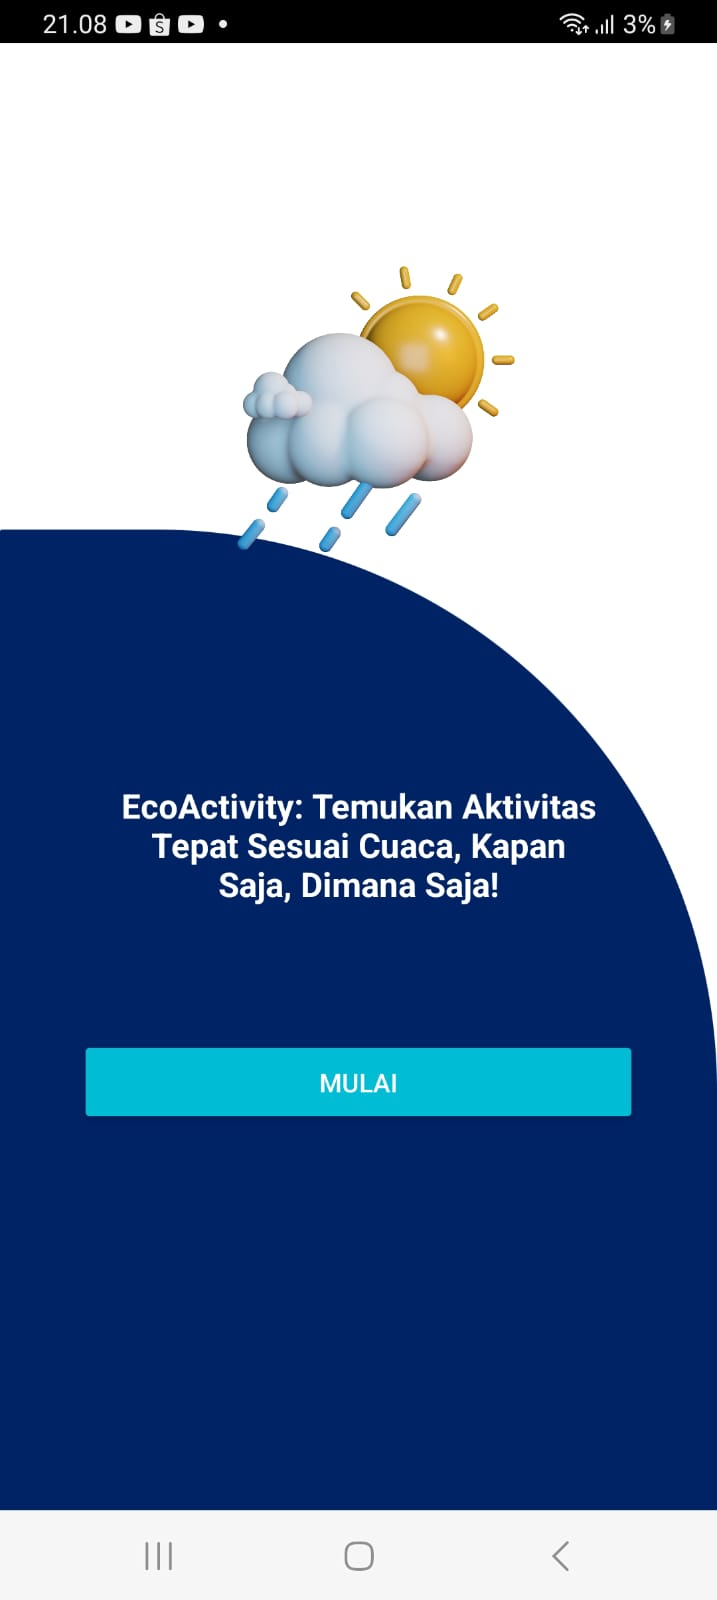
\includegraphics[width=0.6\textwidth]{Definitions/images/01.jpeg}
    \caption{Tampilan halaman utama aplikasi EcoActivity.}
    \label{fig:main-page}
\end{figure}

\begin{figure}[H]
    \centering
    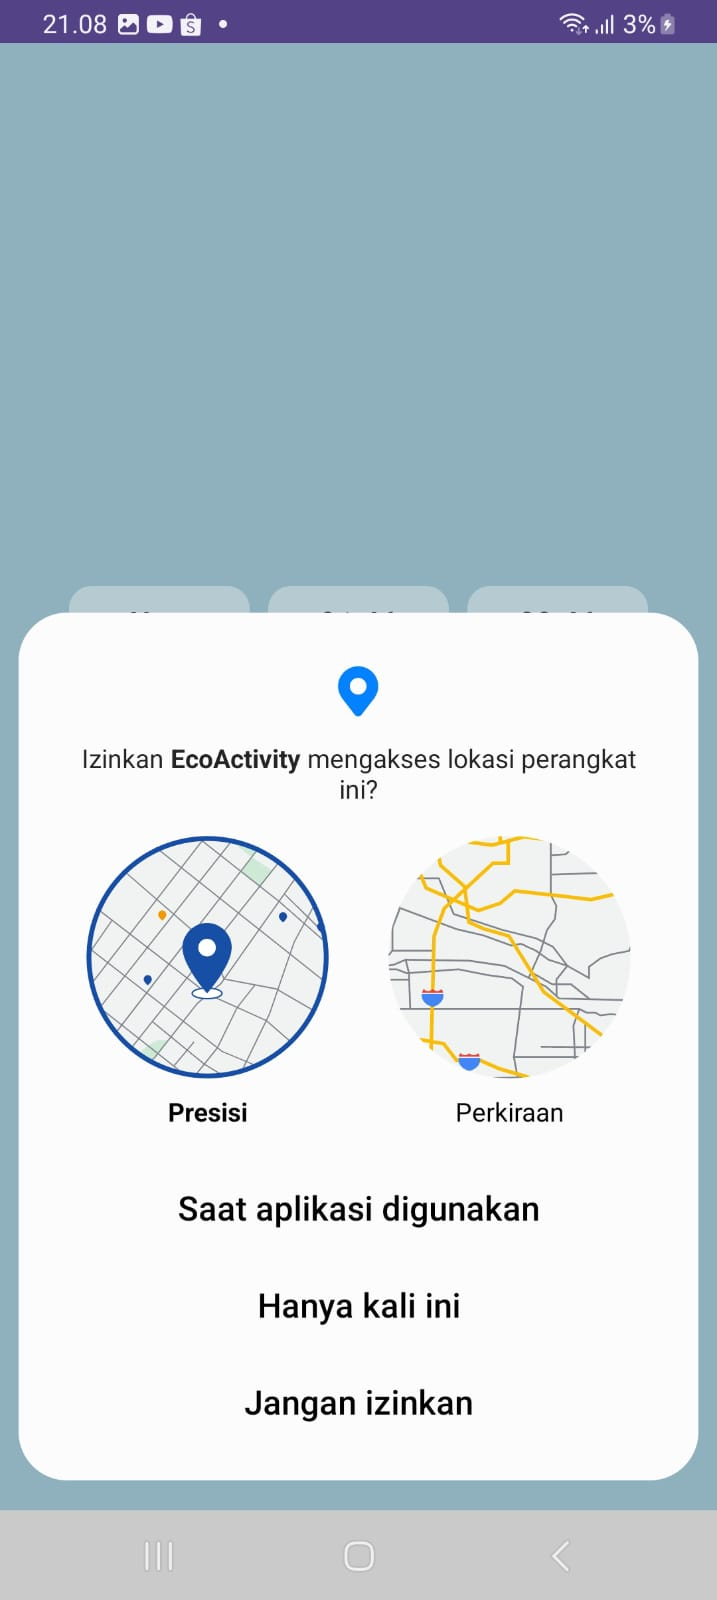
\includegraphics[width=0.6\textwidth]{Definitions/images/02.jpeg}
    \caption{Tampilan halaman lokasi.}
    \label{fig:user-profile}
\end{figure}

\begin{figure}[H]
    \centering
    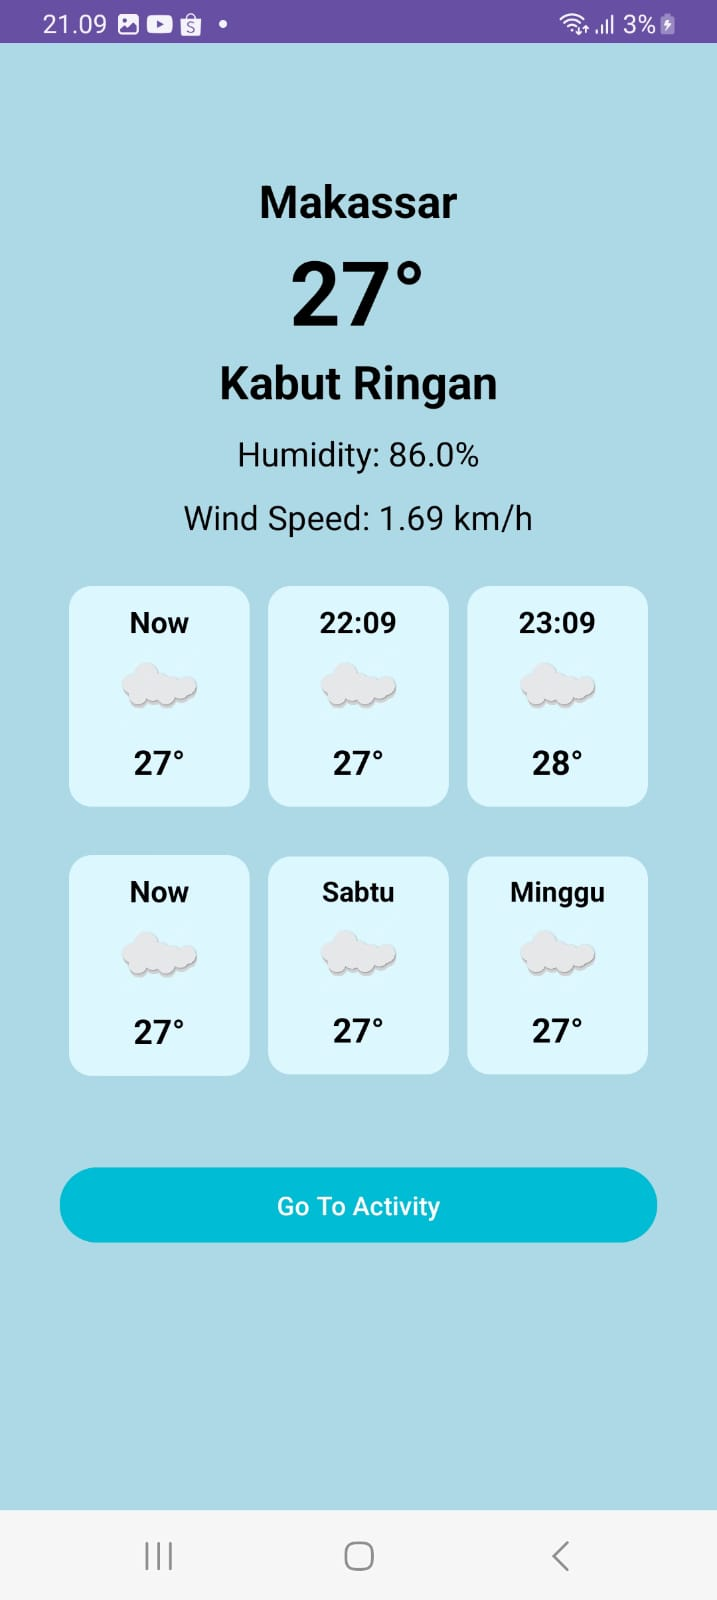
\includegraphics[width=0.6\textwidth]{Definitions/images/03.jpeg}
    \caption{Tampilan halaman informasi cuaca.}
    \label{fig:activity-tracking}
\end{figure}

\begin{figure}[H]
    \centering
    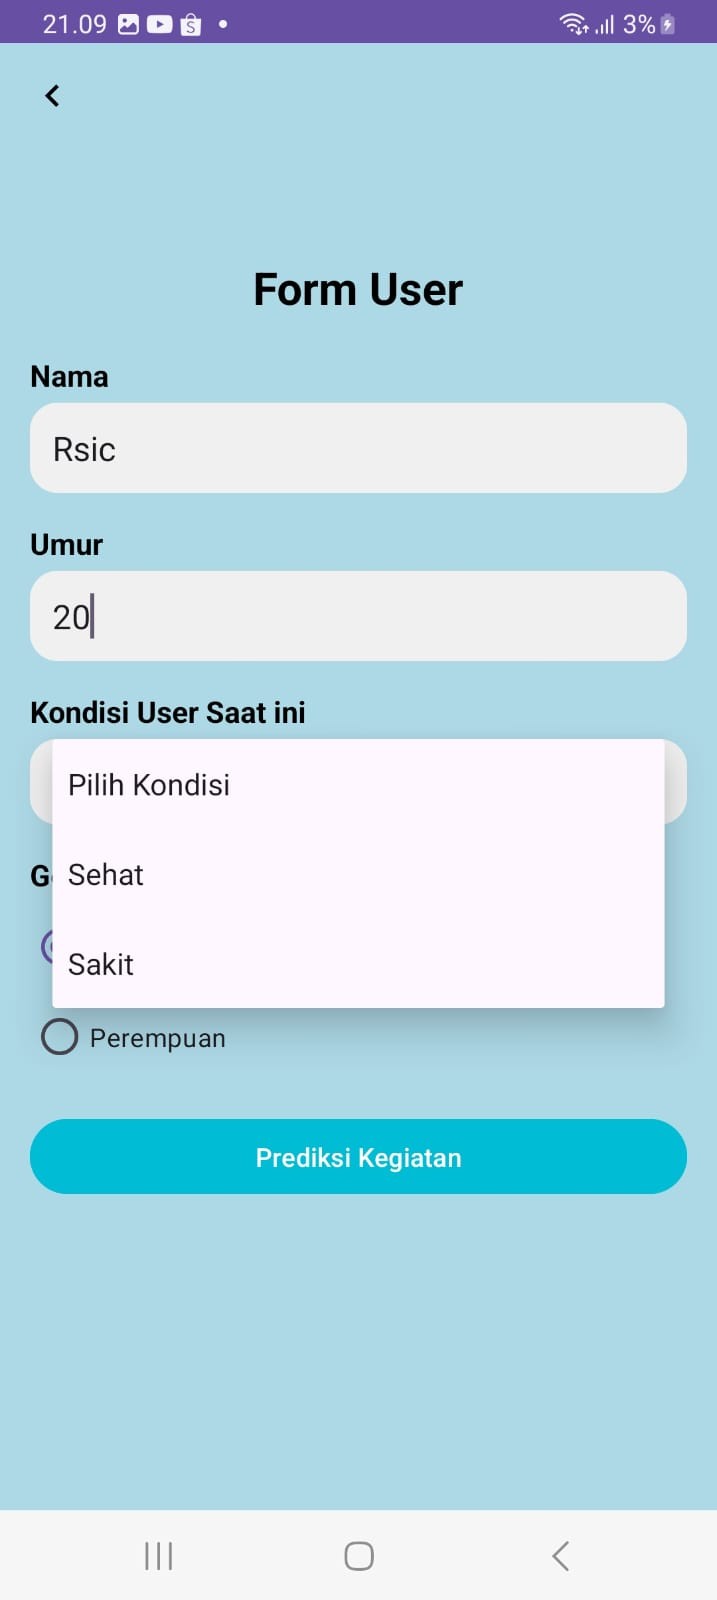
\includegraphics[width=0.6\textwidth]{Definitions/images/04.jpeg}
    \caption{Tampilan fitur kondisi user.}
    \label{fig:stats}
\end{figure}

\begin{figure}[H]
    \centering
    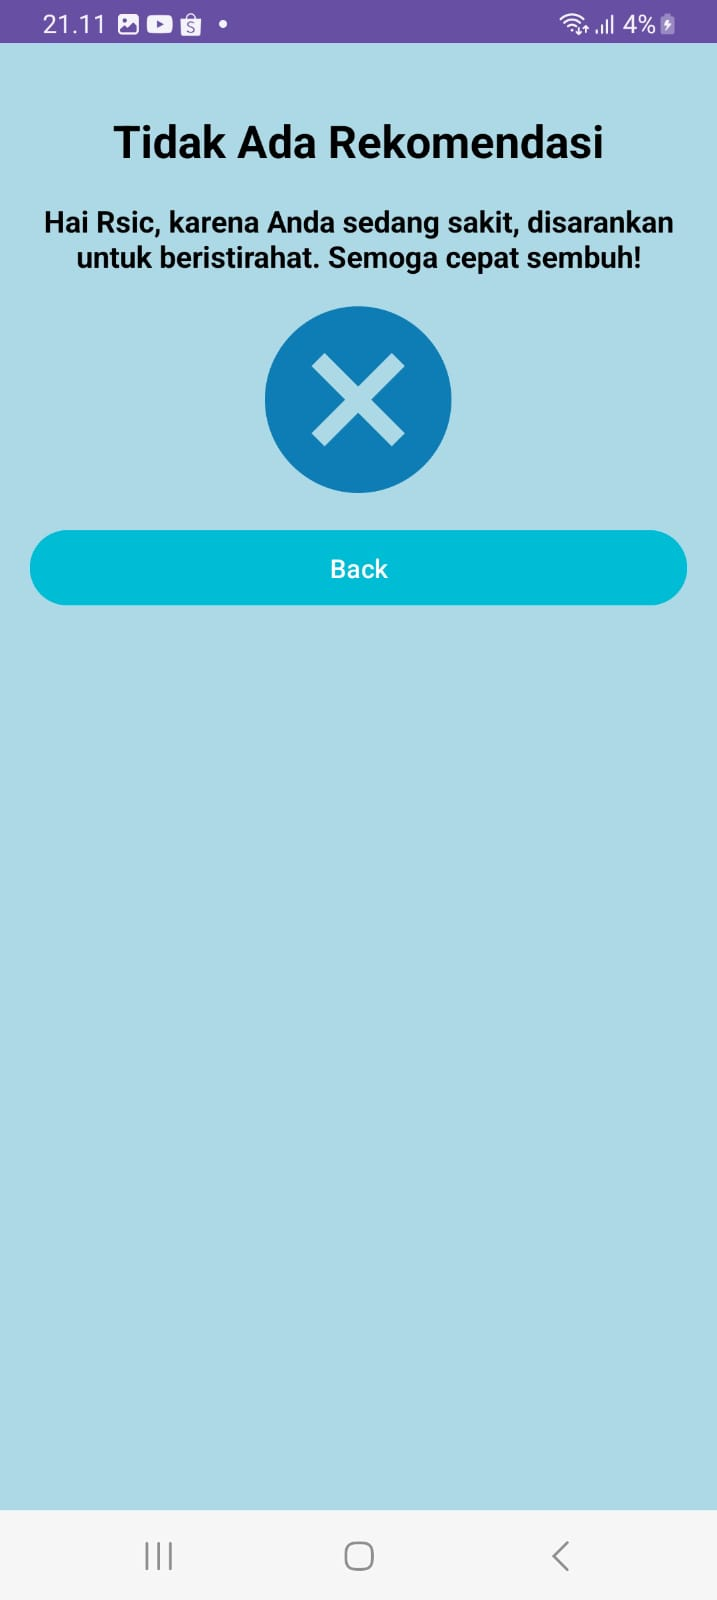
\includegraphics[width=0.6\textwidth]{Definitions/images/05.jpeg}
    \caption{Tampilan halaman user sakit.}
    \label{fig:daily-notifications}
\end{figure}

\begin{figure}[H]
    \centering
    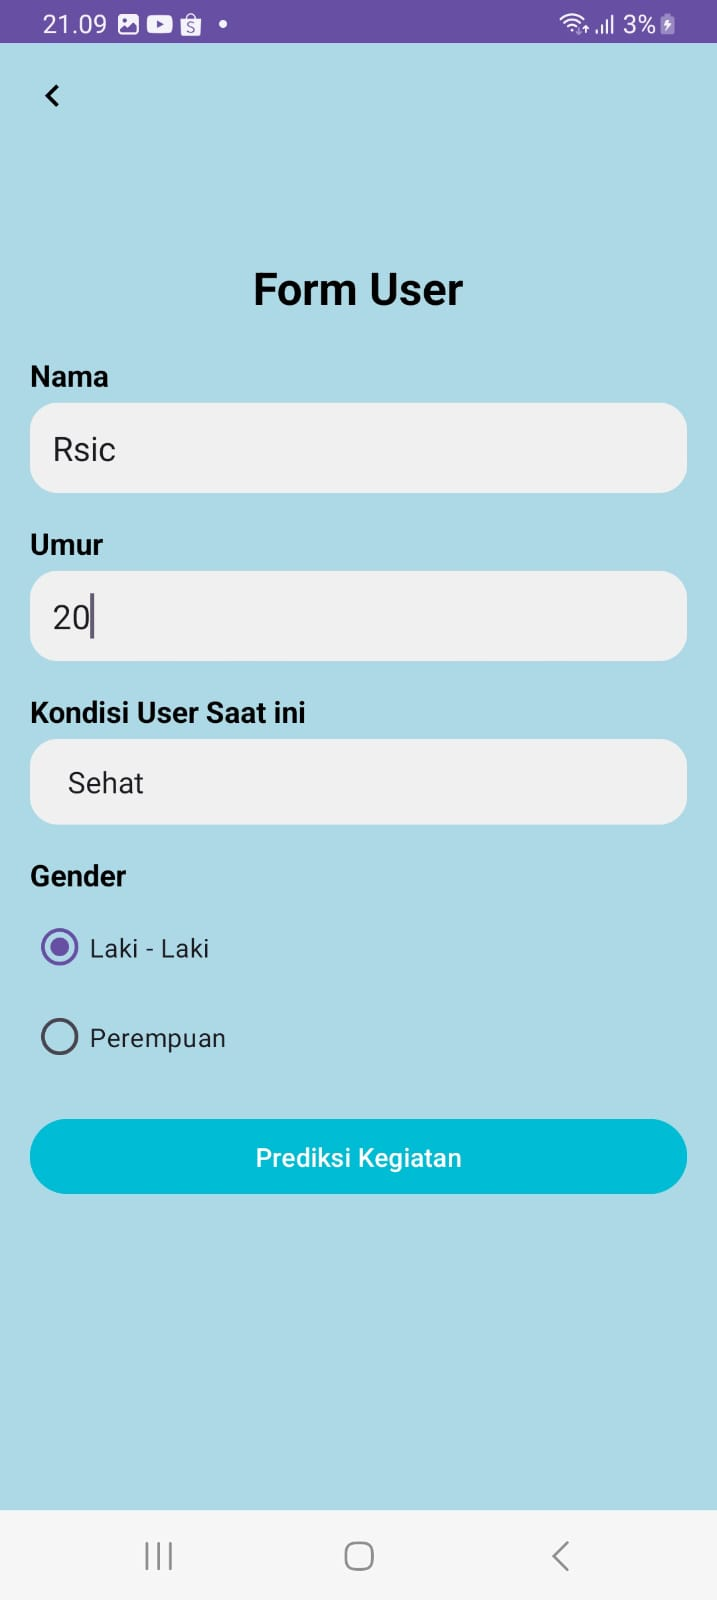
\includegraphics[width=0.6\textwidth]{Definitions/images/06.jpeg}
    \caption{Tampilan fitur kondisi user.}
    \label{fig:settings}
\end{figure}

\begin{figure}[H]
    \centering
    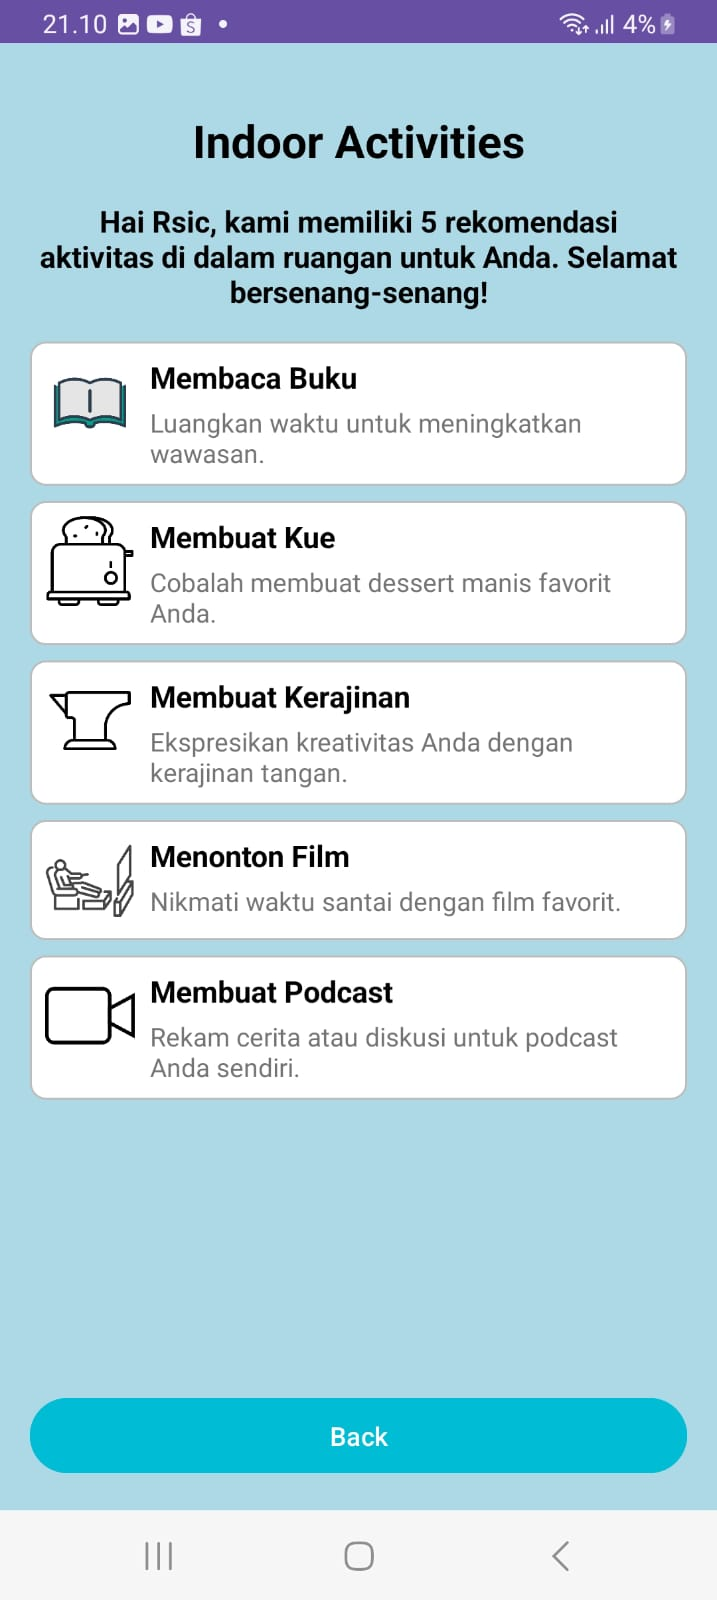
\includegraphics[width=0.6\textwidth]{Definitions/images/07.jpeg}
    \caption{Tampilan halaman kondisi sehat.}
    \label{fig:help-page}
\end{figure}


\subsubsection{API Integration}
API Tomorrow diintegrasikan untuk mendapatkan data cuaca real-time yang diproses di backend untuk memberikan prediksi apakah aktivitas yang sesuai adalah indoor atau outdoor berdasarkan kondisi cuaca terkini. API ini menyediakan data seperti suhu, kelembapan, kecepatan angin, dan kondisi cuaca (cerah, hujan, dll.), yang digunakan untuk menentukan jenis aktivitas yang relevan.

\subsubsection{Activity Prediction Model}
Sistem ini tidak menggunakan model prediksi cuaca berbasis data historis. Sebagai gantinya, menggunakan algoritma berbasis aturan untuk memprediksi apakah aktivitas yang sesuai adalah indoor atau outdoor. Berdasarkan data cuaca real-time yang diperoleh dari API, sistem akan mengkategorikan aktivitas sesuai dengan kondisi cuaca, dan memberikan daftar aktivitas yang relevan (misalnya outdoor untuk cuaca cerah dan indoor untuk cuaca hujan).

\subsubsection{User Interface (UI)}
Antarmuka pengguna dibangun di Android Studio dan dirancang untuk memberikan pengalaman yang intuitif. Tampilan utama mencakup informasi cuaca terkini serta daftar aktivitas yang relevan berdasarkan prediksi indoor/outdoor. Pengguna dapat dengan mudah melihat rekomendasi aktivitas berdasarkan kondisi cuaca saat itu.

\subsubsection{Backend Functionality}
Backend berfungsi untuk mengelola data dari API Tomorrow dan memproses informasi cuaca untuk menentukan kategori aktivitas (indoor atau outdoor). Backend juga menyimpan preferensi pengguna, yang memungkinkan aplikasi memberikan rekomendasi yang lebih dipersonalisasi berdasarkan data cuaca terkini dan preferensi pengguna sebelumnya.
\section{Results and Discussion}

\subsubsection{Hasil Evaluasi Sistem Prediksi Indoor/Outdoor}

Sistem EcoActivity memberikan Prediksi Indoor/Outdoor berdasarkan kondisi cuaca real-time yang diperoleh dari API. Evaluasi dilakukan untuk memeriksa seberapa baik sistem ini dapat mengklasifikasikan apakah aktivitas yang sesuai adalah indoor atau outdoor, berdasarkan data cuaca saat ini.

\begin{figure}[htbp]
    \centering
    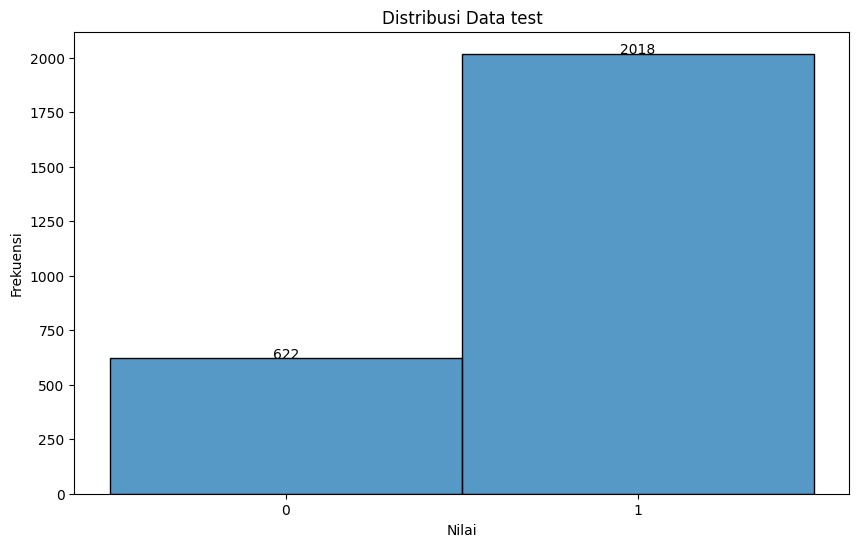
\includegraphics[width=0.8\textwidth]{Definitions/images/1.jpeg}
    \caption{Distribusi data awal menunjukkan ketidakseimbangan antara kelas 0 dan 1, dengan kelas 1 mendominasi. Hal ini dapat menyebabkan bias pada model pembelajaran mesin.}
    \label{fig:distribusi_awal}
\end{figure}

\begin{figure}[H]
    \centering
    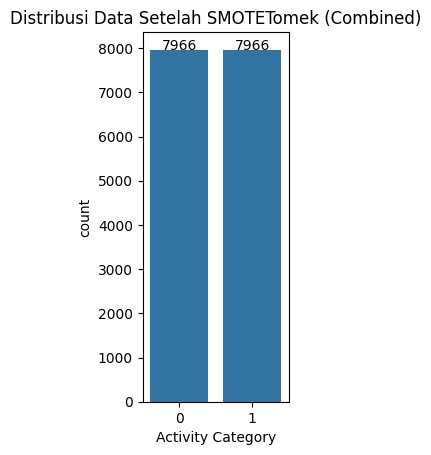
\includegraphics[width=0.6\textwidth]{Definitions/images/2.jpeg}
    \caption{Distribusi data setelah proses SMOTETomek menunjukkan keseimbangan antara kelas 0 dan 1. Teknik ini menggabungkan oversampling dengan undersampling untuk menangani ketidakseimbangan data.}
    \label{fig:distribusi_resampling}
\end{figure}

\begin{figure}[H]
    \centering
    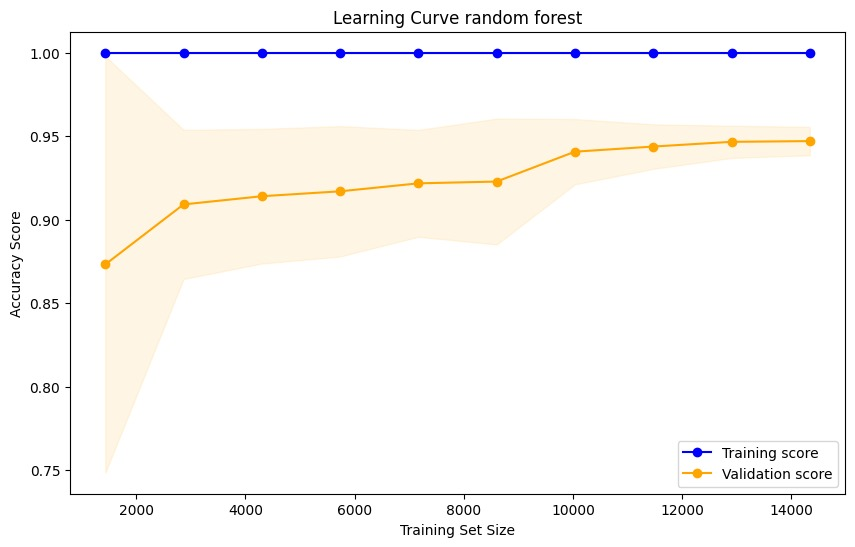
\includegraphics[width=0.6\textwidth]{Definitions/images/3.jpeg}
    \caption{Classification report sebelum optimasi}
\end{figure}

\begin{figure}[H]
    \centering
    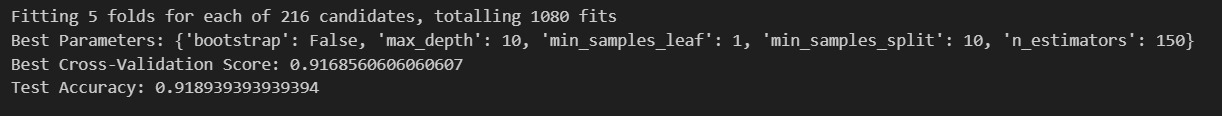
\includegraphics[width=0.6\textwidth]{Definitions/images/6.jpeg}
    \caption{Classification report setelah optimasi}
\end{figure}

\begin{figure}[H]
    \centering
    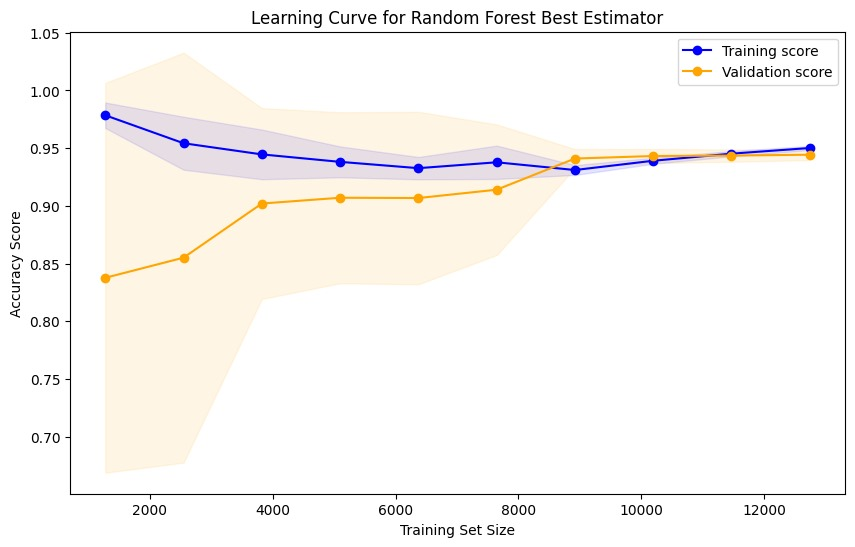
\includegraphics[width=0.6\textwidth]{Definitions/images/4.jpeg}
    \caption{Score awal sebelum hyperparameter.}
\end{figure}

\begin{figure}[H]
    \centering
    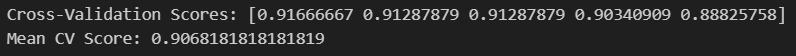
\includegraphics[width=0.6\textwidth]{Definitions/images/5.jpeg}
    \caption{Hasil setelah optimasi model dengan hyperparameter.}
\end{figure}
\begin{figure}[H]
    \centering
    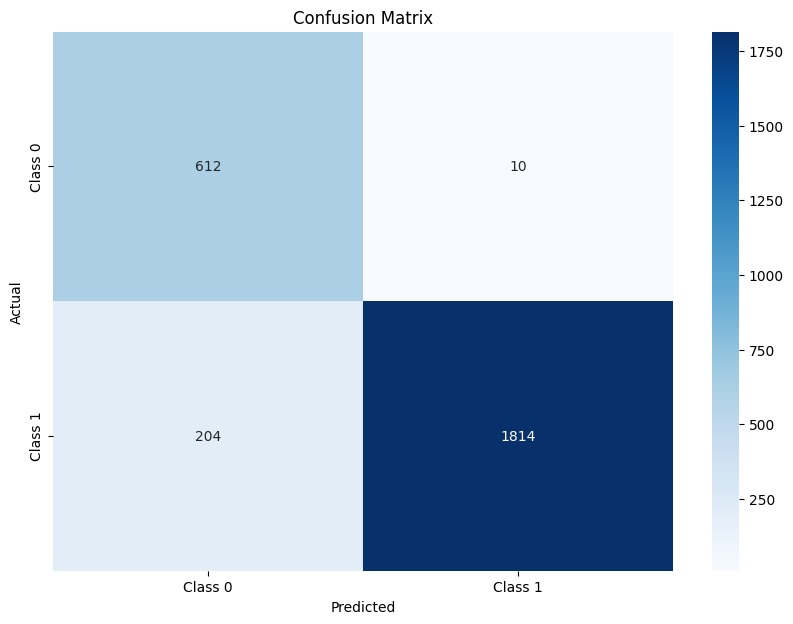
\includegraphics[width=0.6\textwidth]{Definitions/images/7.jpeg}
    \caption{Confusion matrix}
    \label{fig:heatmap_confusion}
\end{figure}

Tabel berikut menunjukkan hasil evaluasi berdasarkan akurasi sistem dalam memberikan rekomendasi aktivitas indoor atau outdoor berdasarkan kondisi cuaca yang diterima dari API:

\begin{table}[h]
    \centering
    \caption{Classification Report dari Sistem Prediksi Indoor/Outdoor}
    \begin{tabular}{lcccc}
        \hline
        Kelas & Precision & Recall & F1-Score & Support \\
        \hline
        0 (Outdoor) & 0.75 & 0.98 & 0.85 & 622 \\
        1 (Indoor) & 0.99 & 0.90 & 0.94 & 2018 \\
        \hline
        \textbf{Accuracy} & \multicolumn{4}{c}{0.92 (Total: 2640)} \\
        Macro Avg & 0.87 & 0.94 & 0.90 & 2640 \\
        Weighted Avg & 0.94 & 0.92 & 0.92 & 2640 \\
        \hline
    \end{tabular}
    \label{tab:indoor-outdoor-classification}
\end{table}

Hasil evaluasi ini menunjukkan bahwa sistem berhasil mengklasifikasikan aktivitas indoor dan outdoor dengan akurasi 0.92. F1-score untuk kategori Outdoor adalah 0.85, sementara untuk kategori Indoor adalah 0.94. Dengan hasil ini, aplikasi EcoActivity menunjukkan kinerja yang baik dalam memberikan rekomendasi aktivitas yang sesuai berdasarkan kondisi cuaca terkini.
\subsection{Discussion}
Kendala yang ditemukan selama pengujian mencakup latensi pada jaringan yang lambat dan akurasi prediksi yang dapat ditingkatkan dengan dataset yang lebih besar atau model yang lebih canggih.

\section{Conclusion}

Aplikasi EcoActivity berhasil mengintegrasikan data cuaca real-time dengan daftar aktivitas yang disesuaikan berdasarkan kondisi cuaca terkini. Menggunakan Tomorrow API untuk memperoleh informasi cuaca real-time, aplikasi ini dapat memberikan daftar aktivitas indoor atau outdoor yang relevan, tergantung pada kondisi cuaca yang terjadi saat ini. Dengan menggunakan dataset Aktivitas dan Parameter Cuaca, aplikasi ini dilatih untuk memprediksi apakah aktivitas yang sesuai harus dilakukan di dalam ruangan atau luar ruangan, berdasarkan parameter cuaca seperti suhu, kelembapan, kecepatan angin, dan lainnya.

Hasil evaluasi menunjukkan bahwa aplikasi dapat memberikan daftar aktivitas yang tepat sesuai dengan kondisi cuaca, yang memungkinkan pengguna merencanakan kegiatan dengan lebih efektif. Ke depan, pengembangan aplikasi dapat difokuskan pada peningkatan keakuratan dan personalisasi, seperti memberikan daftar aktivitas berdasarkan lokasi atau preferensi pengguna, untuk meningkatkan pengalaman dan efisiensi aplikasi EcoActivity dalam menyediakan informasi yang relevan bagi pengguna.
\end{document}

